\chapter{Fundamentação teórica}

Este capítulo aborda os conceitos teóricos necessários para a compreensão do presente trabalho.

\section{Aprendizado de Máquina}

O aprendizado de máquina é um subcampo da inteligência artificial que tem por objetivo o desenvolvimento de algoritmos capazes de aprender e tomar decisões a partir de um conjunto de dados, sem que seja necessária a programação explícita para essas tarefas específicas \cite{mlDietterich}. Fundamentalmente, esses sistemas buscam aprender padrões em coleções de dados para, a partir da generalização desse conhecimento, realizar inferências sobre novas informações. Esse processo de aprendizado utiliza modelos matemáticos, principalmente estatísticos, que capturam relações complexas entre variáveis de entrada e saída através do ajuste de parâmetros internos, permitindo que a aplicação melhore seu desempenho conforme é exposta a mais dados \cite{mlSarker}. Em geral, as técnicas de \textit{machine learning} são categorizadas em três paradigmas principais: aprendizagem supervisionada, não supervisionada e por reforço.

O aprendizado supervisionado caracteriza-se pela utilização de conjuntos de dados rotulados, onde tanto as entradas quanto as saídas desejadas são conhecidas durante o treinamento. Nesse paradigma, o algoritmo aprende através de exemplos, de forma a possibilitar tarefas como classificação — a atribuição de classes discretas aos dados — e regressão — a predição de valores contínuos. Algoritmos clássicos dessa categoria incluem máquinas de vetores de suporte, redes neurais artificiais e métodos \textit{ensemble} \cite{mlSarker}. O aprendizado não-supervisionado, por sua vez, opera sobre dados não rotulados, sem o conhecimento das saídas desejadas, e busca compreender a organização natural de um dado conjunto a partir da identificação de padrões intrínsecos. Essa abordagem engloba técnicas como agrupamento (\textit{clustering}) e detecção de anomalias \cite{mlSarker}. Ainda, diferentes estratégias de aprendizado podem ser incorporadas, como algoritmos semi-supervisionados, utilizados quando um \textit{dataset} tem poucos dados classificados, de forma a aproveitar a estrutura implícita do conjunto não categorizado para melhorar o desempenho do modelo \cite{mlSarker}.

Adicionalmente, o aprendizado por reforço representa um paradigma distinto onde um modelo aprende através de interações com um ambiente, sendo recompensado ou penalizado com base em suas ações, de forma que gradualmente desenvolva estratégias ótimas. Essa abordagem é especialmente útil em áreas como teoria de jogos ou inteligência de enxame \cite{mlSarker}.

Embora os conceitos fundamentais de aprendizado de máquina tenham sido estabelecidos há quase um século, com contribuições embrionárias nas décadas de 1950 e 1960 \cite{mlDietterich}, essa área de estudo tem recebido grande destaque nas últimas décadas. Esse ressurgimento deve-se principalmente ao aumento exponencial da capacidade computacional e a disponibilidade massiva de dados digitais. Também, a evolução do \textit{hardware}, particularmente o advento de unidades de processamento gráfico de alto desempenho, possibilitou o treinamento de modelos complexos, antes computacionalmente intratáveis, transformando o aprendizado de máquina em uma tecnologia fundamental para aplicações modernas em diversas áreas \cite{mlSarker}.

\section{Redes Neurais Profundas}

Redes neurais profundas, comumente utilizadas no paradigma de aprendizado supervisionado, são uma especialização de redes neurais artificiais. Diferentemente das técnicas tradicionais de \textit{machine learning}, que requerem a engenharia manual de características, são capazes de autonomamente aprender representações complexas de um determinado conjunto de dados brutos. Isso é possível por sua estrutura multicamada, que permite a extração progressiva de características de baixo nível -- em uma imagem, por exemplo, bordas e linhas -- até padrões de alto nível -- no mesmo exemplo, objetos e faces \cite{efficientdeep}.

A unidade mais básica de uma rede neural artificial é um neurônio artificial (que será referido aqui apenas como neurônio ou nó).

\begin{figure}[H]
	\caption{\label{fig:neuron}Representação de um Neurônio Artificial}
    \begin{center}
    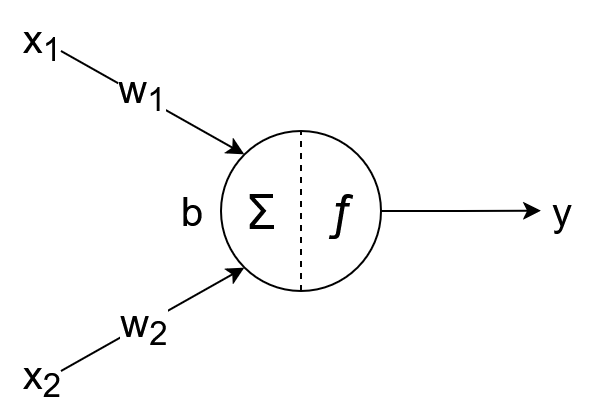
\includegraphics[width=0.7\linewidth]{images/neuron.png}
	\end{center}
	\fonte{o autor}
\end{figure}

No exemplo representado na figura \ref{fig:neuron}, um neurônio recebe dados de entrada, $x_1$ e $x_2$, e produz uma saída $y$. Para isso, cada entrada é multiplicada por seu respectivo peso, $w_1$ e $w_2$, e somada junto a um termo de viés $b$ -- assim, a equação resultante é igual a $\Sigma = x_1*w_1 + x_2*w_2 + b$. Finalmente, aplica-se uma função de ativação $f$ sobre a soma para converter esse valor em um intervalo desejado -- a tangente hiperbólica produziria um número dentro do intervalo $(-1, 1)$, enquanto a sigmoid produziria um intervalo entre $(0, 1)$, por exemplo -- resultando na saída $y$ \cite{deeplearningbook}. Em outras palavras, os pesos indicam a importância, ou força, da conexão entre a entrada e o neurônio; o viés atua como um limiar de ativação que independe das entradas; e a função de ativação transforma uma entrada linear em uma saída não linear, o que permite um mapeamento complexo entre entradas e saídas. 

Uma rede neural artificial é formada pela interligação de neurônios, assim, uma camada da rede é denominada a partir de um grupo de nós interligados, que processam dados de uma maneira específica. Combinando uma camada de entrada, camadas intermediárias e uma camada de saída, obtém-se uma rede neural profunda, ilustrada na figura \ref{fig:dnn}. Dessa forma, cada camada recebe entradas ponderadas a partir das camadas anteriores, aplicam uma função de ativação e propagam o resultado para as camadas subsequentes \cite{deeplearningbook}. Diferentes configurações destas, como a variação das conexões entre neurônios ou o emprego de funções de ativação distintas, tem por efeito especializações, ou habilidades de aprendizado específicas, assim, a utilização de múltiplas camadas permite a assimilação de representações hierárquicas complexas. \cite{reviewdeep}.

\begin{figure}[H]
	\caption{\label{fig:dnn}Representação de um Neurônio Artificial}
    \begin{center}
    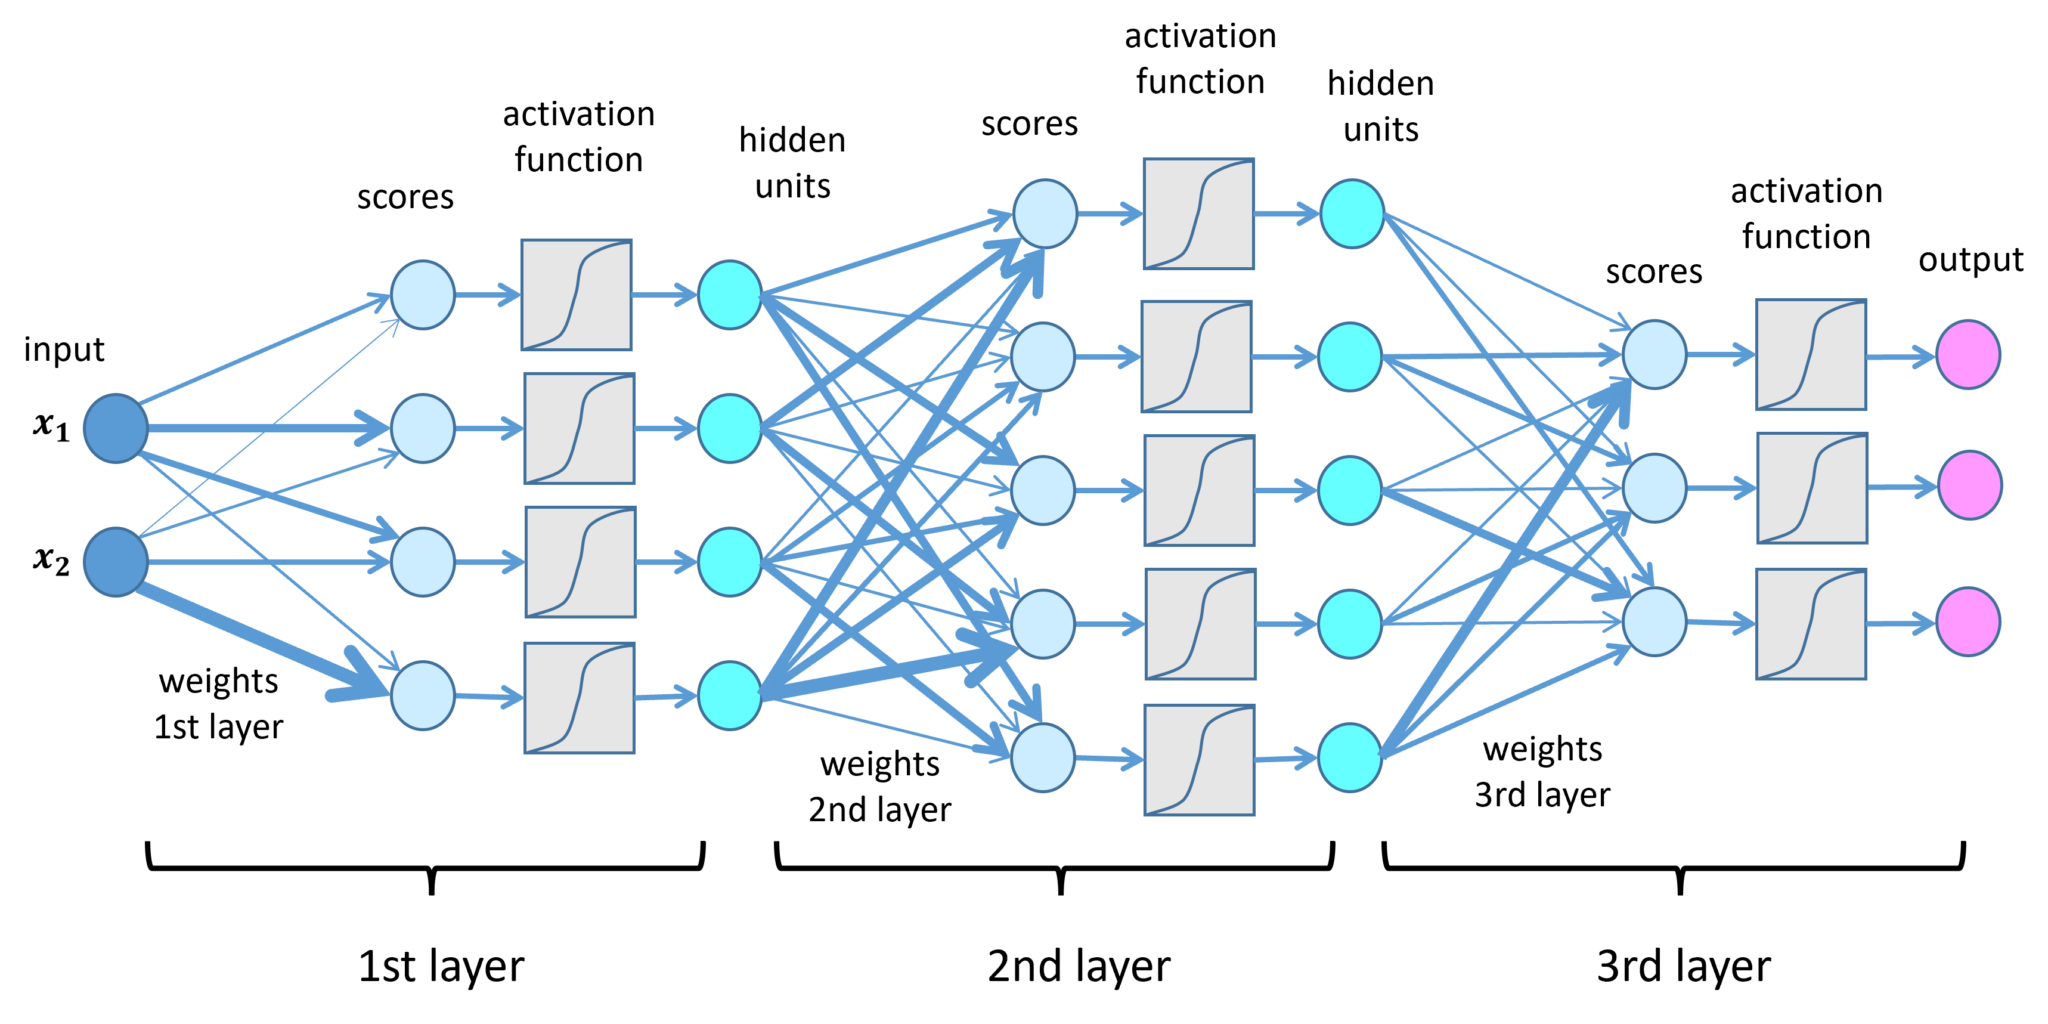
\includegraphics[width=1\linewidth]{images/dnn.png}
	\end{center}
	\fonte{\url{https://lamarr-institute.org/blog/deep-neural-networks/}. Acesso em: 25 junho 2025}
\end{figure}


O processo de aprendizado da rede é denominado treinamento e consiste na estimação e ajuste dos parâmetros através de um algoritmo de retropropagação. Seu objetivo é calcular o gradiente de uma função que mede o erro entre o valor de saída computado e o esperado, além de ajustar os pesos e vieses dos neurônios na direção oposta ao gradiente, para minimizar o erro. Esse processo é executado em cada camada, propagando o erro desde a camada de saída até a de entrada, de forma iterativa, por múltiplas épocas, até que a rede converja para uma solução otimizada \cite{deeplearningbook}, como ilustrado na figura \ref{fig:gradientdescent}, em que o eixo $y$ representa valores de erro e o eixo $x$ valores de peso.

\begin{figure}[H]
	\caption{\label{fig:gradientdescent}Visualização do Gradiente Descendente}
    \begin{center}
    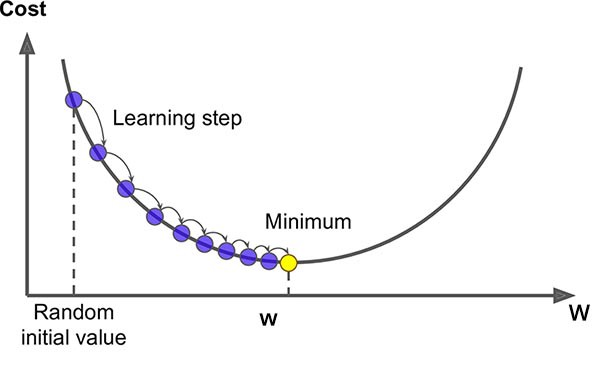
\includegraphics[width=1\linewidth]{images/gradientdescent.jpg}
	\end{center}
	\fonte{\url{https://mlpills.dev/machine-learning/gradient-descent/}. Acesso em: 25 junho 2025}
\end{figure}


\subsection{Redes Neurais Convolucionais}

\subsubsection{Reconhecimento Óptico de Caracteres}

\subsection{Processamento de Linguagem Natural}

\section{Análise Multimodal}

\section{Aprendizado não-supervisionado}

\subsection{Algoritmos de Agrupamento}

% K-means, DBSCAN, HDBSCAN aplicados a documentos

\subsection{Detecção de Anomalias e Outliers}

% detecção de outliers e anomalias